\documentclass[11pt]{article}

\usepackage{fontspec}
\usepackage[a4paper,margin=1in]{geometry}
\usepackage{amsmath}
\usepackage{graphicx}
\usepackage{booktabs}
\usepackage{tabularx}
\usepackage{xcolor}
\usepackage{microtype}
\usepackage[font=small,labelfont=bf]{caption}
\usepackage{enumitem}
\usepackage{tikz}
\usetikzlibrary{arrows.meta,positioning}
\usepackage[colorlinks=true,linkcolor=accent,citecolor=accent,urlcolor=accent]{hyperref}

\definecolor{accent}{HTML}{2459A8}
\definecolor{zfill}{HTML}{EEF2F8}
\definecolor{zline}{HTML}{2A78D6}
\definecolor{muted}{HTML}{7D838F}
\definecolor{hl}{HTML}{FBE1D6}

\hypersetup{
  pdftitle={Probing a Tor-network style to anonymize a model in LLM usage},
  pdfauthor={LaumerLoma},
  pdfsubject={Model attribution under multi-hop rewriting},
  pdfkeywords={LLM, authorship attribution, anonymity, onion routing},
}

\setlist{itemsep=2pt,topsep=4pt}
\emergencystretch=1.5em
\newcommand{\cond}[1]{\texttt{#1}}
\newcommand{\ci}[2]{\,[#1,\,#2]}

\title{\textbf{Probing a Tor-network style to anonymize\\a model in LLM usage}}
\author{LaumerLoma}
\date{October 2026}

\begin{document}
\maketitle

\begin{abstract}
\noindent
Readers can often tell which language model wrote a piece of text. We test whether routing an answer through a circuit of other models hides the source model, $Z$. $Z$ first answers a nested ``telephone'' prompt. The answer is then rewritten in turn by an exit, a middle and a guard model, each drawn at random from five labs. Against an adaptive attacker that knows the scheme and trains on its outputs, a style classifier identifies $Z$ \textbf{87.5\%} of the time without protection and \textbf{28.5\%} after the full circuit (chance is 20\%). A variant where the relays exist only as personas inside $Z$'s prompt makes $Z$ \emph{easier} to identify (93.2\%). A single rewrite by a random model reaches 42.8\%. The signal that remains is concentrated in one model. An exploratory follow-up on a larger second run (800 units) finds that attackers which never see the wording, only length, layout and named facts, come within 1--4 points of the best wording-based attacker, while surviving three-word phrases do not predict which answers get attributed. Answers lose about half their length on the way through. The protocol and hypotheses were fixed before data collection.
\end{abstract}

\section{Introduction}

A model's output carries its fingerprints: favourite openings, list habits, hedging phrases, formatting and length. Simple classifiers pick these up reliably. Sometimes that is unwanted. Examples include blind comparisons, products that want provider-neutral output, and any setting where the reader's opinion of a model should not colour how they read the answer.

The design was inspired by Tor \cite{tor}, which routes traffic through a \emph{guard}, a \emph{middle} and an \emph{exit} relay. We borrow only the shape and the names, combined with the children's game of telephone. The prompt goes forward through a chain of named intermediaries, and the answer comes back through the same chain, each hop restating it. Unlike Tor, the chain gives no cryptographic guarantee. Any protection has to come from the rewriting itself, which makes the scheme a form of authorship obfuscation. Whether it changes what an attacker can infer is an empirical question, and the answer depends on how the hops are implemented.

\noindent This report makes three contributions:
\begin{enumerate}
  \item A pre-registered measurement of how well the source model can be attributed under six variants of the scheme, using two attacker families and attackers that adapt to the scheme.
  \item Evidence that persona framing on its own does not anonymize. Real hops through other models are what reduce attribution.
  \item A breakdown of the signal that remains: it is uneven across models, survives even when only meaning is used as a feature, and in an exploratory follow-up is almost fully reachable from length, layout and facts, without the wording.
\end{enumerate}

\section{Related work}
\label{sec:related}

\paragraph{Identifying the source model.} Outputs of different LLMs are easy to tell apart. Sun et al.\ \cite{idiosyncrasies} fine-tune text-embedding models to reach 97.1\% accuracy on five-way attribution between frontier chat models. Shuffling the words costs little accuracy, which locates much of the signal in word choice. Most relevant here, they report that the signal survives when another LLM rewrites, translates or summarises the text, which suggests that it is partly carried by content. LLMmap \cite{llmmap} studies an active version of the problem, sending a few crafted queries to an application and identifying 42 model versions with over 95\% accuracy from eight interactions. That threat is stronger than ours, since our adversary only reads text it is given.

\paragraph{Provider-side attribution.} Watermarking embeds a statistical signal in generated tokens so that the provider can later detect its own output \cite{watermark}. Paraphrasing weakens such signals, and paraphrasing by other models is known to evade AI-text detectors more generally \cite{dipper,sadasivan}. Our relays are paraphrasers in this sense. We do not test watermarks, because none of our local models produce them.

\paragraph{Authorship obfuscation.} Hiding a human author's identity by rewriting their text has a long history. Brennan et al.\ \cite{adversarial-stylometry} showed that people imitating another writer's style defeat stylometric classifiers. The PAN shared tasks on author obfuscation \cite{pan2017,pan2018} formalised the evaluation along three axes: \emph{safety} (can the author still be identified?), \emph{soundness} (is the meaning preserved?) and \emph{sensibleness} (does the text read naturally?). Our attribution accuracy measures safety. Our utility measure is a coarse proxy for soundness, and we do not measure sensibleness.

\paragraph{Rewriting with a language model for privacy.} DP-Prompt \cite{dpprompt} paraphrases a document with a pretrained LLM through zero-shot prompting and controls the privacy--utility trade-off through the sampling temperature, which yields a local differential-privacy guarantee. It distinguishes \emph{static} from \emph{adaptive} attackers, as we do, and finds that adaptive attackers recover much of the author signal: author-identification F1 drops by 46\% against static attackers but only 26\% against adaptive ones. Our setting differs in what is hidden (the model rather than a human author) and in the use of several hops through different models. We borrow its temperature baseline.

\paragraph{Anonymous communication.} Onion routing \cite{tor} protects the link between sender and receiver through layered encryption, so that no single relay sees both ends. Our scheme borrows its vocabulary only. Each relay sees the full text, and anonymity depends entirely on how well the rewriting removes the source model's signal.

\section{The scheme}
\label{sec:scheme}

Five labs act as nodes. For each query, the guard ($A$), middle ($B$) and exit ($C$) are drawn uniformly \emph{without replacement}, and $Z$'s own lab can be drawn. Excluding it would leak information: an attacker could then rule out whichever lab spoke last. $Z$ receives one forward prompt:

\begin{quote}\small\ttfamily\raggedright
Tell me a version of what \{A\} would return if it asked \{B\} what \{C\} would say about the following. [\ldots] Reply only with the final answer \{A\} would give, in plain prose.
\end{quote}

The return path comes in two forms. In \textbf{Z-relay} mode (the scheme as first specified), $Z$ makes one more call that restates its own answer ``as $A$ would return it after $B$ relayed $C$'s answer''. The relays exist only as names inside $Z$'s prompts. In \textbf{node-relay} mode, the exit, middle and guard models each rewrite the answer with their \emph{own} weights, using a neutral ``restate this in your own words, keep every fact'' prompt. A regular-expression scrubber runs last and removes self-identifying sentences and lab or model names. Figure~\ref{fig:scheme} shows the conditions we measure. The full relay prompts are in Appendix~\ref{app:prompts}.

\begin{figure}[t]
\centering
\resizebox{\linewidth}{!}{%
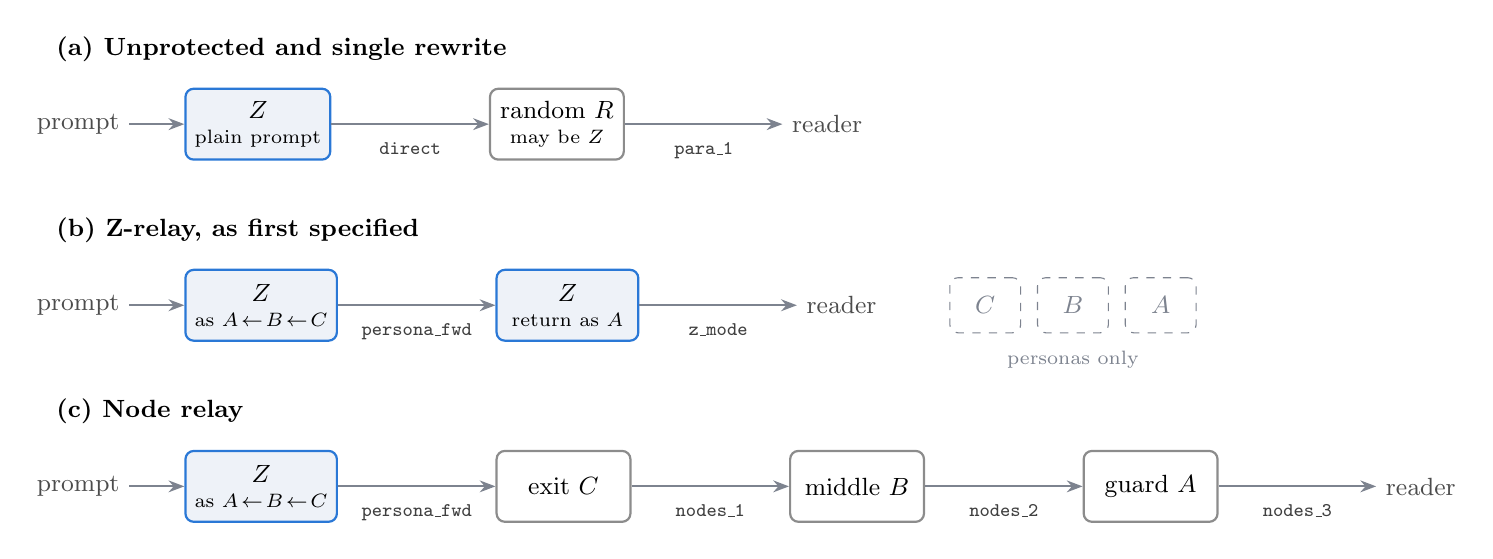
\begin{tikzpicture}[
  font=\small,
  node distance=7mm,
  every node/.style={align=center},
  zbox/.style={draw=zline, fill=zfill, thick, rounded corners=3pt, minimum height=9mm, minimum width=18mm},
  real/.style={draw=black!45, thick, rounded corners=3pt, minimum height=9mm, minimum width=17mm},
  virt/.style={draw=muted, dashed, rounded corners=3pt, minimum height=7mm, minimum width=9mm, text=muted},
  io/.style={text=black!70},
  arr/.style={-{Stealth[length=2mm]}, thick, draw=muted},
  tag/.style={font=\scriptsize\ttfamily, below=3pt, text=black!75},
  lane/.style={font=\small\bfseries, anchor=west},
]
% (a) unprotected and one rewrite
\node[lane] at (0,0.95) {(a) Unprotected and single rewrite};
\node[io] (p1) at (0.4,0) {prompt};
\node[zbox, right=of p1] (z1) {$Z$\\[-2pt]\scriptsize plain prompt};
\node[real, right=20mm of z1] (r1) {random $R$\\[-2pt]\scriptsize may be $Z$};
\node[io, right=20mm of r1] (o1) {reader};
\draw[arr] (p1) -- (z1);
\draw[arr] (z1) -- node[tag] {direct} (r1);
\draw[arr] (r1) -- node[tag] {para\_1} (o1);

% (b) z-relay
\node[lane] at (0,-1.35) {(b) Z-relay, as first specified};
\node[io] (p2) at (0.4,-2.3) {prompt};
\node[zbox, right=of p2] (z2a) {$Z$\\[-2pt]\scriptsize as $A\!\leftarrow\!B\!\leftarrow\!C$};
\node[zbox, right=20mm of z2a] (z2b) {$Z$\\[-2pt]\scriptsize return as $A$};
\node[io, right=20mm of z2b] (o2) {reader};
\draw[arr] (p2) -- (z2a);
\draw[arr] (z2a) -- node[tag] {persona\_fwd} (z2b);
\draw[arr] (z2b) -- node[tag] {z\_mode} (o2);
\node[virt, right=8mm of o2] (vc) {$C$};
\node[virt, right=2mm of vc] (vb) {$B$};
\node[virt, right=2mm of vb] (va) {$A$};
\node[font=\scriptsize, text=muted, below=1mm of vb] {personas only};

% (c) node relay
\node[lane] at (0,-3.65) {(c) Node relay};
\node[io] (p3) at (0.4,-4.6) {prompt};
\node[zbox, right=of p3] (z3) {$Z$\\[-2pt]\scriptsize as $A\!\leftarrow\!B\!\leftarrow\!C$};
\node[real, right=20mm of z3] (c3) {exit $C$};
\node[real, right=20mm of c3] (b3) {middle $B$};
\node[real, right=20mm of b3] (a3) {guard $A$};
\node[io, right=20mm of a3] (o3) {reader};
\draw[arr] (p3) -- (z3);
\draw[arr] (z3) -- node[tag] {persona\_fwd} (c3);
\draw[arr] (c3) -- node[tag] {nodes\_1} (b3);
\draw[arr] (b3) -- node[tag] {nodes\_2} (a3);
\draw[arr] (a3) -- node[tag] {nodes\_3} (o3);
\end{tikzpicture}}
\caption{The measured conditions, read left to right. Blue boxes are calls to $Z$, grey boxes are calls to another lab's model, and dashed boxes are personas that exist only inside $Z$'s prompt. Labels under the arrows mark where each condition is taken. \cond{nodes\_1}--\cond{nodes\_3} are intermediate states of one chain.}
\label{fig:scheme}
\end{figure}

\section{Experimental setup}

The protocol, hypotheses and analysis were written down before any real-model data was collected. Nothing was changed afterwards.

\paragraph{Threat model.} The adversary sees only the final text. It knows the scheme and the five candidate models, and it can generate as much labelled training data as it likes by running the scheme itself, following Kerckhoffs's principle \cite{kerckhoffs}. Providers, who see all traffic, are out of scope, as are network observers and timing.

\paragraph{Models and prompts.} Each lab is represented by one small instruct model served locally through LM Studio: Meta (Llama~3.2 3B), Google (Gemma~3 4B), Alibaba (Qwen3 4B 2507), Microsoft (Phi-4-mini) and Mistral AI (Ministral~3 3B). Every call uses temperature 0.7 and a 400-token limit. There are 80 fixed prompts across explanation, advice, coding, maths, creative writing, opinion and factual questions. Every model plays $Z$ for every prompt, giving \textbf{400 units}. Circuits are drawn from a seed fixed for each unit. The full run makes 2{,}880 model calls.

\paragraph{Attackers.} Two feature sets feed an $\ell_2$-regularised logistic regression with the regularisation strength chosen by inner cross-validation. \emph{Style}: TF-IDF of character 2--5-grams plus word 1--2-grams. \emph{Meaning}: nomic-embed-text-v1.5 sentence embeddings \cite{nomic}. The \emph{adaptive} attacker trains and tests on the same condition, which is the attacker the threat model calls for. The \emph{static} attacker trains on unprotected answers only. All evaluation uses 5-fold cross-validation \emph{grouped by prompt}, so no prompt appears in both training and test data. 95\% intervals come from 2{,}000 bootstrap resamples over prompts.

\paragraph{Utility.} Utility is the cosine similarity between the embedding of the final text and that of $Z$'s unprotected answer to the same prompt. Two reference points calibrate it. The \emph{floor} is the similarity between two different models' unprotected answers to the same prompt (0.914). The \emph{ceiling} is the similarity between two samples from the same model (0.954).

\section{Results}

\subsection{Attribution under each condition}

Without protection, the style attacker attributes 87.5\% of answers correctly (Figure~\ref{fig:accuracy}, Table~\ref{tab:accuracy}). The meaning attacker is far weaker (54.8\%): small models answer the same question with similar content, and what separates them is how they write. Persona framing alone lowers style attribution only slightly (78.8\%). The Z-relay return pass \emph{raises} it to 93.2\%. Once a real model sits between $Z$ and the reader, accuracy falls sharply. Three hops bring it down to 28.5\%\ci{24.8}{32.5}. The interval stays clear of chance.

\begin{figure}[t]
\centering
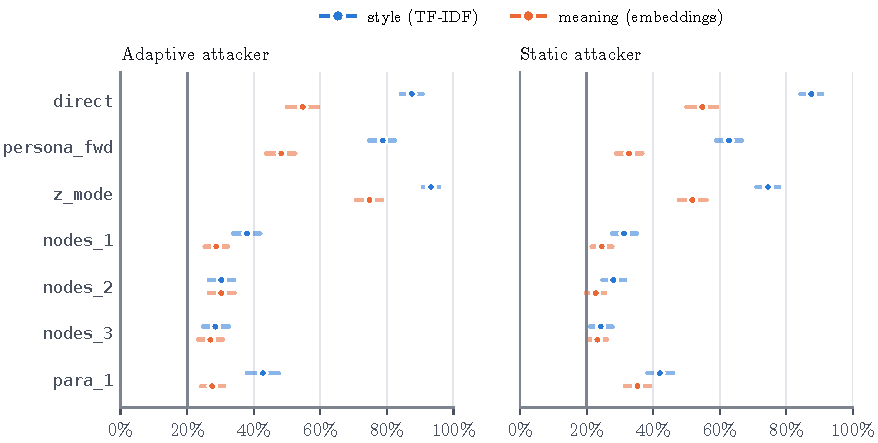
\includegraphics[width=\linewidth]{figures/accuracy.pdf}
\caption{Attribution accuracy by condition, with 95\% bootstrap intervals over prompts. The vertical rule marks chance (20\%). The static attacker never saw protected text during training. For \cond{direct} the two attackers are the same.}
\label{fig:accuracy}
\end{figure}

\begin{table}[t]
\centering
\small
\begin{tabular}{@{}l rrrr r@{}}
\toprule
 & \multicolumn{2}{c}{Style (TF-IDF)} & \multicolumn{2}{c}{Meaning (embeddings)} & \\
\cmidrule(lr){2-3}\cmidrule(lr){4-5}
Condition & adaptive & static & adaptive & static & $\to$guard \\
\midrule
\cond{direct}      & \textbf{87.5}\ci{84.2}{90.8} & --- & 54.8\ci{50.0}{59.3} & --- & --- \\
\cond{persona\_fwd} & 78.8\ci{74.8}{82.5} & 62.7\ci{59.0}{66.8} & 48.2\ci{43.8}{52.5} & 32.8\ci{28.7}{36.8} & 4 \\
\cond{z\_mode}      & \textbf{93.2}\ci{90.8}{95.8} & 74.5\ci{71.0}{77.8} & 74.8\ci{70.8}{78.5} & 51.7\ci{47.8}{56.0} & 2 \\
\cond{nodes\_1}     & 38.0\ci{33.8}{42.0} & 31.2\ci{27.8}{35.0} & 28.7\ci{25.2}{32.2} & 24.5\ci{21.5}{27.8} & 13 \\
\cond{nodes\_2}     & 30.2\ci{26.5}{34.0} & 28.0\ci{24.8}{31.5} & 30.2\ci{26.5}{34.2} & 22.8\ci{19.8}{25.5} & 12 \\
\cond{nodes\_3}     & \textbf{28.5}\ci{24.8}{32.5} & 24.2\ci{21.0}{27.8} & 27.0\ci{23.2}{30.8} & 23.2\ci{20.8}{26.0} & 19 \\
\cond{para\_1}      & 42.8\ci{38.0}{47.5} & 42.0\ci{38.2}{46.0} & 27.5\ci{24.2}{31.0} & 35.2\ci{31.5}{39.0} & --- \\
\bottomrule
\end{tabular}
\caption{Attribution accuracy in \%, with 95\% CIs. Chance is 20\%. ``$\to$guard'' is the share of the adaptive style attacker's predictions that name the guard lab, counted on units where the guard is not $Z$.}
\label{tab:accuracy}
\end{table}

\subsection{What each hop does}

The first independent hop does most of the work: style attribution falls from 78.8\% after $Z$'s forward answer to 38.0\% after the exit rewrites it (Figure~\ref{fig:hops}a). The middle and guard hops add a further 9.5 points between them. The static attacker shows the mechanism. Trained on unprotected answers, it increasingly names the \emph{guard} lab instead of $Z$, reaching 35\% after the third hop (Figure~\ref{fig:hops}b). The final text mostly carries the last relay's voice.

\begin{figure}[t]
\centering
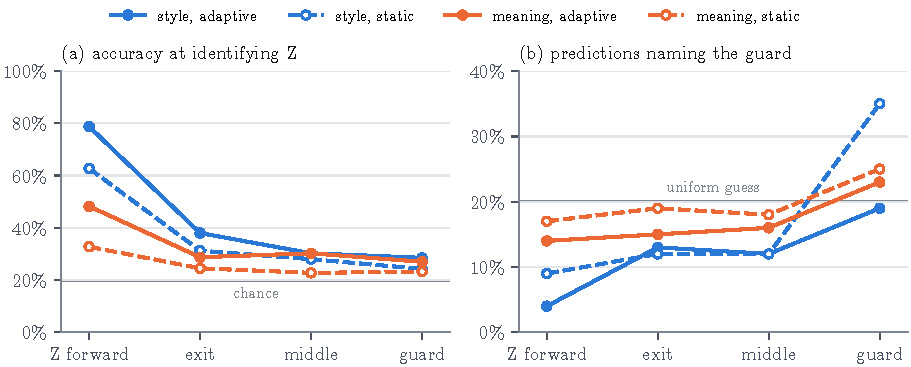
\includegraphics[width=\linewidth]{figures/hops.pdf}
\caption{One node-relay chain, hop by hop. (a) Accuracy at identifying $Z$; the reference line is chance. (b) Share of predictions that name the guard lab, on units where the guard is not $Z$; the reference line is what uniform guessing would score.}
\label{fig:hops}
\end{figure}

\subsection{Who still leaks}

Without protection, every model except Alibaba's is recognised in at least 7 of 8 units (Figure~\ref{fig:confusion}a). After three hops the diagonal mostly dissolves, but not evenly. Meta and Microsoft sit at 29\% each, Alibaba at 20\% and Google at 16\%. Mistral is still recognised in 39 of 80 units (49\%). Much of the remaining signal is one model's, and the risk depends on which model is $Z$.

\begin{figure}[t]
\centering
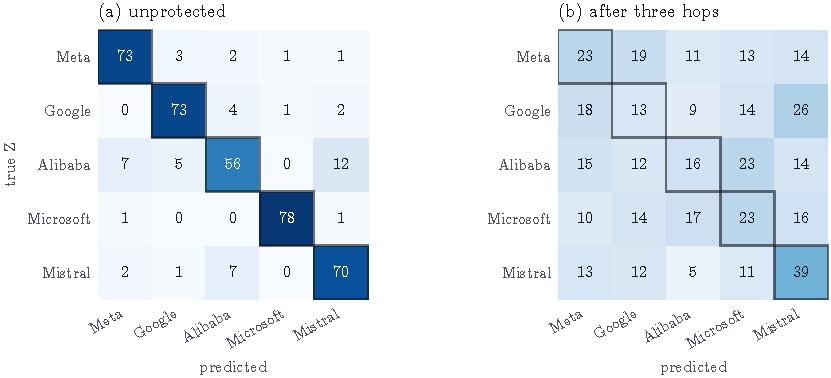
\includegraphics[width=\linewidth]{figures/confusion.pdf}
\caption{Confusion matrices for the adaptive style attacker. Rows are the true $Z$, columns the predicted model, and each row sums to 80. Outlined cells are correct predictions.}
\label{fig:confusion}
\end{figure}

\subsection{Privacy against utility}

Every condition that uses the persona prompt ends up \emph{further} from $Z$'s plain answer than another model's plain answer is: cosine similarity is 0.868--0.892, against a floor of 0.914 (Figure~\ref{fig:utility}). The nested prompt changes the answer before any hop does: it compresses it and changes its focus. Answers shrink from 246 words to 124 after three hops (Table~\ref{tab:utility}). The single random rewrite (\cond{para\_1}) stays at the noise ceiling, so it keeps the meaning, but it leaks more style. Embedding similarity cannot tell rewording apart from lost content. It bounds utility loosely and does not measure it precisely.

\begin{figure}[t]
\centering
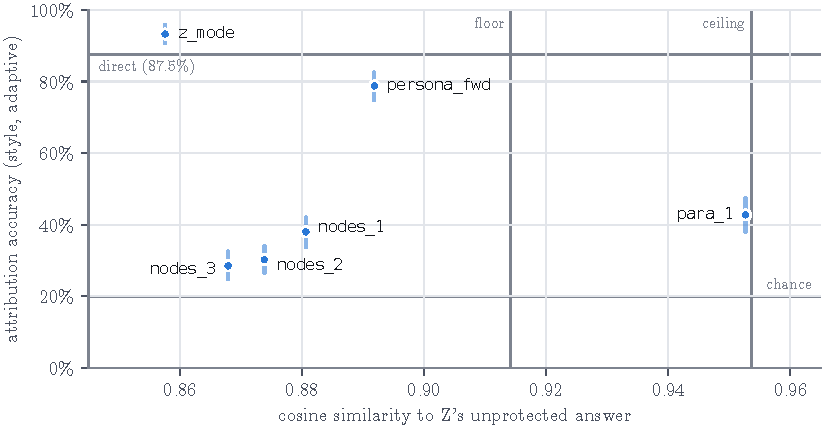
\includegraphics[width=\linewidth]{figures/utility.pdf}
\caption{Each condition placed by how similar its output is to $Z$'s unprotected answer (x) and how often the adaptive style attacker identifies $Z$ (y). Bars are 95\% intervals. Vertical rules mark the floor (two different models) and the ceiling (the same model resampled). The ideal sits bottom right.}
\label{fig:utility}
\end{figure}

\begin{table}[t]
\centering
\small
\begin{tabular}{@{}lrrrrrrr@{}}
\toprule
 & \cond{direct} & \cond{persona\_fwd} & \cond{z\_mode} & \cond{nodes\_1} & \cond{nodes\_2} & \cond{nodes\_3} & \cond{para\_1} \\
\midrule
cosine to \cond{direct} & --- & 0.892 & 0.858 & 0.881 & 0.874 & 0.868 & 0.953 \\
mean words & 246 & 169 & 200 & 138 & 126 & 124 & 197 \\
\bottomrule
\end{tabular}
\caption{Utility and mean length. Reference points: floor 0.914 (two different models), ceiling 0.954 (same model resampled).}
\label{tab:utility}
\end{table}

\subsection{Hypotheses}

A hypothesis counts as supported only if the interval meets the stated condition. Table~\ref{tab:hyp} lists the six pre-registered hypotheses and their verdicts.

\begin{table}[t]
\centering
\small
\begin{tabularx}{\linewidth}{@{}l >{\raggedright\arraybackslash}X l >{\raggedright\arraybackslash}X@{}}
\toprule
 & Prediction (fixed before data collection) & Verdict & Evidence \\
\midrule
H1 & \cond{direct} is highly attributable, $\geq 70\%$ & Supported & 87.5\%\ci{84.2}{90.8} \\
H2 & Z-relay lowers accuracy but stays above chance & \textbf{Rejected} & 93.2\%\ci{90.8}{95.8}, above \cond{direct} \\
H3 & The full circuit is lower than Z-relay & Supported & 28.5\% vs.\ 93.2\% \\
H4 & The full circuit still beats chance & Supported & lower bounds 24.8\% (style), 23.2\% (meaning) \\
H5 & One random rewrite $\approx$ the full circuit & \textbf{Not supported} & style 42.8\%\ci{38.0}{47.5} vs.\ 28.5\%\ci{24.8}{32.5}; meaning CIs overlap \\
H6 & Utility falls with each hop & Consistent & $0.881 \to 0.874 \to 0.868$; no interval computed \\
\bottomrule
\end{tabularx}
\caption{Pre-registered hypotheses and outcomes.}
\label{tab:hyp}
\end{table}

\section{A worked example}

Table~\ref{tab:example} traces ``Why is the sky blue?'' with Alibaba's model as $Z$. The circuit drew Alibaba as the exit, Google as the middle and Meta as the guard. $Z$'s unprotected answer opens with a bolded term and a bulleted list. The forward pass already turns it into three sentences of plain prose. Each hop then rewords it and keeps the physics. The highlighted phrase is absent from the exit's version but appears at the middle hop. It matches $Z$'s original answer, but the middle model never saw that answer. Relays do not only reword. They draw on their own knowledge, despite the instruction to add nothing.

\begin{table}[t]
\centering
\small
\renewcommand{\arraystretch}{1.25}
\begin{tabularx}{\linewidth}{@{}p{2.35cm} X@{}}
\toprule
Stage & Text (scrubbed) \\
\midrule
\cond{direct}\newline{\footnotesize $Z$, 196 words} & The sky appears blue due to a phenomenon called \textbf{Rayleigh scattering}. Here's a simple explanation: $\bullet$ Sunlight (white light) is made up of different colors, each with its own wavelength. Shorter wavelengths (like blue and violet) scatter more easily than longer wavelengths (like red and yellow) when they hit molecules in the atmosphere. [\ldots] \\
\cond{persona\_fwd}\newline{\footnotesize $Z$, forward} & The sky appears blue because molecules in the atmosphere scatter blue light more than other colors of light. This scattering happens when sunlight enters the atmosphere, and shorter wavelengths like blue and violet are scattered in all directions by air molecules. Our eyes perceive this scattered blue light, which is why the sky looks blue during the day. \\
\cond{nodes\_1}\newline{\footnotesize exit: Alibaba} & The sky appears blue due to the way molecules in the atmosphere scatter sunlight. When sunlight enters the atmosphere, shorter wavelength colors such as blue and violet are scattered more effectively than other colors. This scattered light reaches our eyes from all directions, resulting in the perception of a blue sky during the day. \\
\cond{nodes\_2}\newline{\footnotesize middle: Google} & Sunlight entering Earth's atmosphere is scattered by air molecules. Blue and violet light, possessing shorter wavelengths, are scattered significantly more than other colors \colorbox{hl}{like red and yellow}. Because of this preferential scattering, the blue light is dispersed across the sky, giving it its characteristic color. \\
\cond{nodes\_3}\newline{\footnotesize guard: Meta} & Light from the sun enters Earth's atmosphere and is scattered by air molecules. The light with shorter wavelengths, specifically blue and violet, gets scattered much more than the other colors like red and yellow. This preferential scattering causes the blue light to be spread across the sky, giving it that distinctive color. \\
\bottomrule
\end{tabularx}
\caption{One unit traced through the node-relay chain. The \cond{direct} answer is truncated.}
\label{tab:example}
\end{table}

\section{Where the remaining signal comes from}
\label{sec:residual}

This section is \textbf{exploratory}. The analyses were chosen after the results above were known and were not pre-registered. They need no new model calls.

\paragraph{Data.} The analyses use a second, larger run with its own pre-registered protocol and a separate results report. It doubles the prompts to 160 (the 80 above plus 80 new ones of the same seven types), giving \textbf{800 units} with the same five models and the same way of drawing circuits. It adds a chain without the persona prompt: \cond{plain\_1}--\cond{plain\_3} pass $Z$'s \emph{unprotected} answer through the same exit, middle and guard models as \cond{nodes\_1}--\cond{nodes\_3}. It also adds a third attacker, a ModernBERT-base classifier fine-tuned for each fold. Below, ``best attacker'' means whichever of the three has the highest adaptive accuracy on that condition: TF-IDF on \cond{nodes\_3} (30.5\%\ci{27.5}{33.5}) and the fine-tuned model on \cond{plain\_3} (29.8\%\ci{26.8}{32.6}). The two three-hop chains are statistically indistinguishable.

\paragraph{One model carries most of the signal.} On \cond{nodes\_3}, the best attacker recognises Mistral in 54.4\%\ci{46.2}{61.9} of its units. The other four models together reach 24.5\%\ci{21.4}{27.7}, close to chance. This repeats the pattern of Figure~\ref{fig:confusion}. On \cond{plain\_3}, Mistral is not special (29.4\%). There the leakage is spread over Google (38.8\%) and Microsoft (35.6\%), while Alibaba falls below chance (15.6\%). Mistral's distinctiveness therefore enters through its persona-prompt answers, not through its plain answers. Accuracy on \cond{nodes\_3} is also higher when $Z$'s own lab is one of the relays (33.1\% against 26.8\%) and when it does the last rewrite (37.3\% against 28.8\%, $n=161$). We did not test these differences, but they suggest that letting $Z$'s lab be drawn, which avoids one leak (Section~\ref{sec:scheme}), opens a smaller one.

\paragraph{Attackers that never see the wording.} We trained four attackers that are denied the text itself, on the same grouped folds. \emph{Length}: word, sentence, character and paragraph counts plus the task type, in a gradient-boosted tree model. \emph{Layout}: length plus counts of lines, bullet and numbered items, headers, bold markers and code blocks, and a refusal flag. \emph{Facts}: TF-IDF over numbers and mid-sentence capitalised words only, in the same logistic regression as the style attacker. \emph{Layout+facts}: both, stacked. Table~\ref{tab:content} shows the result. Without protection, wording matters: the best attacker leads layout by 17 points. After three hops, the gap shrinks to 1--4 points, and for layout and layout+facts the paired 95\% interval of the difference includes zero. Nearly all of the accuracy that survives three hops is available without any phrasing. The two kinds of attacker only partly agree on \emph{which} units they get right: when a content-only attacker is right on a three-hop text, the best attacker is also right 38--46\% of the time, against about 30\% if the two were independent.

\begin{table}[t]
\centering
\small
\begin{tabular}{@{}l lll@{}}
\toprule
Attacker & \cond{direct} & \cond{nodes\_3} & \cond{plain\_3} \\
\midrule
Best (sees wording) & \textbf{92.1} & \textbf{30.5} & \textbf{29.8} \\
Length only & 54.9\ci{50.7}{59.1} & 24.5\ci{21.8}{27.4} & 22.0\ci{19.1}{24.9} \\
Layout & 74.8\ci{71.1}{78.2} & 26.8\ci{24.0}{29.5} & 27.1\ci{24.1}{30.1} \\
Facts & 54.2\ci{51.1}{57.6} & 27.4\ci{25.4}{29.5} & 25.5\ci{22.8}{28.2} \\
Layout + facts & 71.5\ci{67.6}{75.0} & 26.8\ci{23.8}{29.6} & 28.7\ci{25.2}{32.0} \\
\midrule
Gap to best, layout & $-17.4$\ci{-20.6}{-14.1} & $-3.7$\ci{-7.4}{0.0} & $-2.6$\ci{-6.5}{1.1} \\
Gap to best, layout + facts & $-20.6$\ci{-24.0}{-17.4} & $-3.7$\ci{-7.5}{0.0} & $-1.0$\ci{-4.6}{2.6} \\
\bottomrule
\end{tabular}
\caption{Adaptive accuracy in \% of attackers that never see the wording (exploratory, second run, 800 units). Chance is 20\%. Gaps are paired bootstrap differences over prompts.}
\label{tab:content}
\end{table}

\paragraph{How much of $Z$'s wording survives.} For each final text we measured the share of its word 3-grams, and separately of its content words (stop words removed), that also occur in $Z$'s text before the hops. As a baseline we used the same share measured against the other four models' texts for the same prompt, which captures overlap that any answer to that question would have. Table~\ref{tab:survival} reports the excess over this baseline. Phrasing fades quickly: the 3-gram excess falls from about 15--20 points after one hop to 4--5 after three. Content words fade much more slowly and still exceed the baseline by 16 points after three hops. The two measures also differ in what they predict. The 3-gram excess is the same whether the best attacker is right or wrong (difference $+0.0$\ci{-0.8}{0.7} on \cond{nodes\_3}). The content-word excess is higher when it is right ($+5.0$\ci{3.3}{6.7} points on \cond{nodes\_3}, $+1.8$\ci{0.2}{3.5} on \cond{plain\_3}), and \cond{nodes\_3} accuracy rises from 20\% to 42\% from the lowest to the highest quartile of content-word excess. Mistral's content words survive the most ($+23$ points) and Meta's the least ($+8$).

\begin{table}[t]
\centering
\small
\begin{tabular}{@{}l rrr rrr@{}}
\toprule
 & \multicolumn{3}{c}{Content words} & \multicolumn{3}{c}{Word 3-grams} \\
\cmidrule(lr){2-4}\cmidrule(lr){5-7}
Condition & own & excess & trace-back & own & excess & trace-back \\
\midrule
\cond{nodes\_1} & 51.8 & $+26.7$ & 83.8 & 18.2 & $+14.9$ & 82.6 \\
\cond{nodes\_2} & 45.6 & $+20.6$ & 79.9 & 10.8 & $+7.8$ & 79.2 \\
\cond{nodes\_3} & 39.9 & $+15.7$ & 70.2 & 6.8 & $+4.4$ & 68.2 \\
\cond{plain\_1} & 60.0 & $+29.7$ & 93.6 & 24.3 & $+20.5$ & 91.8 \\
\cond{plain\_2} & 49.3 & $+19.9$ & 87.8 & 11.0 & $+7.9$ & 80.8 \\
\cond{plain\_3} & 45.6 & $+16.1$ & 83.1 & 7.9 & $+5.0$ & 72.0 \\
\bottomrule
\end{tabular}
\caption{Survival of $Z$'s text, in \%. ``Own'' is the share of the final text's items found in $Z$'s pre-hop text, and ``excess'' is that share minus the mean share found in the other four models' texts for the same prompt (all excess intervals exclude zero). ``Trace-back'' is how often the final text overlaps most with $Z$'s own pre-hop text among the five candidates.}
\label{tab:survival}
\end{table}

\paragraph{A stronger attacker.} The trace-back column hints at a threat the classifiers miss. An attacker who holds all five models' answers to the same prompt can match a three-hop text to its source 68--83\% of the time by word overlap alone, against 30\% for the best classifier. This figure is optimistic, because it uses the exact texts $Z$ produced. A real attacker would have to query each model again and would get different samples, so the true accuracy of this attack is unknown. It is the most important open measurement.

\paragraph{Reading.} After three hops, the signal that survives is mostly \emph{what} was said and how much of it, not \emph{how} it was phrased: length, layout and content words carry it, and exact phrases do not. Two caveats keep this from being a clean split. Layout sits between content and style, since bullets against prose is partly a habit. Content-word overlap includes word choice, which is also partly style. The fact extractor is crude. What the analysis does show is that more rewriting of the same kind is unlikely to remove what is left, because rewriting is told to keep exactly the features that still identify $Z$.

\section{Discussion}

\paragraph{Protection comes from other models, not from framing.} Asking $Z$ to answer ``as $A$ would, relaying $B$ relaying $C$'' changes the surface of its answer, but $Z$ still writes it, and an attacker who trains on such answers learns $Z$'s persona voice as easily as its plain voice. The Z-relay variant does worse than nothing. A second pass through the same model seems to strengthen its habits. If the scheme is deployed, the hops must be real calls to different models.

\paragraph{The voice is replaced, not hidden.} After the third hop the final text mostly reads as the guard's. That is the intended outcome, and it moves the question to whether anything of $Z$ survives below the surface. Some of it does. The adaptive attacker stays above chance with both feature sets, and the meaning attacker reaches the same accuracy as the style attacker (27.0\% against 28.5\%). The remaining signal is probably in \emph{what} is said: which facts are chosen, how the answer is structured, what is left out. Section~\ref{sec:residual} tests this directly.

\paragraph{Leakage is uneven.} Mistral's answers remain identifiable in half the units. Its long forward answers may be too much for the small relays to restate fully, or its distinctive content may survive restating. Either way, how private a deployment is depends on which model it is protecting.

\paragraph{Cost.} Node relay takes four sequential calls instead of one and halves the length of the answer. One random rewrite is cheaper, keeps more content and gives up about 14 points of attribution accuracy. The persona prompt's compression may be acceptable for chat. For tasks where detail matters, it is a real loss.

\section{Next steps}
\label{sec:next}

\paragraph{Frontier models.} The most important open question is whether any of this holds for frontier models, which may show their identity more strongly and imitate other voices better. The code already supports any OpenAI-compatible router, so the full second-run design can be repeated with five frontier labs: 800 units, ten conditions, plus a second unprotected sample per unit for the re-query attack above, \textbf{8{,}800 calls} in all. On the local run these used 2.55M input and 2.64M output tokens. Frontier models write longer answers, so if every output fills the 400-token cap the totals rise to about 3.1M input and 3.5M output tokens. Table~\ref{tab:cost} turns these volumes into cost at standard API prices as listed on 12 October 2026.

\begin{table}[t]
\centering
\small
\setlength{\tabcolsep}{4pt}
\begin{tabular}{@{}l l r l r@{}}
\toprule
 & \multicolumn{2}{c}{Flagship tier} & \multicolumn{2}{c}{Mid tier} \\
\cmidrule(lr){2-3}\cmidrule(lr){4-5}
Lab & model & \$ in / out & model & \$ in / out \\
\midrule
Anthropic & Claude Opus 5.5 & 4 / 20 & Claude Sonnet 5.5 & 2 / 10 \\
OpenAI & GPT-6 Astra & 10 / 50 & GPT-6.1 Sol & 2 / 10 \\
Google & Gemini 3.1 Pro & 2 / 12 & Gemini 3.8 Flash & 0.75 / 3.75 \\
xAI & Grok 4.7 & 2 / 6 & Grok 4.3 & 1.25 / 2.50 \\
DeepSeek & DeepSeek V4 Pro & 0.435 / 0.87 & DeepSeek V4 Flash & 0.14 / 0.28 \\
\midrule
Run, measured lengths & & \$51 & & \$15 \\
Run, outputs at 400-token cap & & \$67 & & \$20 \\
Fixed rewriter (\cond{fixed\_1}) & & +\$0.4--20 & & +\$0.1--4 \\
+1{,}000 reasoning tokens/call & & +\$156 & & +\$47 \\
\bottomrule
\end{tabular}
\caption{Estimated cost of repeating the second run with frontier models, in US dollars, with prices per million tokens. Calls are spread evenly over the five labs, except \cond{fixed\_1}, whose cost depends on which lab is the fixed rewriter (cheapest to most expensive). Prices were taken from the providers' pricing pages on 12 October 2026, except DeepSeek's, which come from its documentation as quoted by a search result. The Gemini 3.8 Flash price is introductory until 31 December 2026, and the DeepSeek V4 Pro price may be a temporary discount.}
\label{tab:cost}
\end{table}

The token bill itself is small: about \$50--90 for flagship models and \$15--25 for mid-tier ones. Hidden reasoning tokens are the main risk to the budget, because they are billed as output. At 1{,}000 reasoning tokens per call they would raise the flagship cost three- to fourfold, so reasoning should be switched off or set to its minimum. That also keeps the relays closer to plain rewriters. Batch APIs, which Anthropic, OpenAI and Google offer at half price, suit the staged collection and would cut the cost further. Lifting the 400-token cap would raise the cost roughly in proportion to the longer answers. The attackers run locally and add no API cost. With such a small budget, several samples per unit, more prompts or an LLM-judge attacker are affordable as well.

\paragraph{Other steps.} Three further experiments follow from Section~\ref{sec:residual}.
\begin{enumerate}
  \item \emph{Separate content from style directly.} Reduce each answer to a list of facts and rebuild it with one fixed model before the hops, which should remove style and leave content. Conversely, give all five models the same list of facts to write up, which leaves only style.
  \item \emph{Normalise length and layout.} Ask every relay for a fixed length and plain prose, and measure how much of the remaining signal this removes and what it costs in utility.
  \item \emph{Re-query attack.} Repeat the trace-back attack with fresh samples of each model's answer, which is the version a real attacker could run.
\end{enumerate}

\section{Limitations}

\begin{itemize}
  \item \textbf{Small models.} All five models have 3--4B parameters. Frontier models may show their identity more strongly and may imitate other voices better, so the results may move in either direction.
  \item \textbf{Two attacker families.} A fine-tuned transformer classifier or an LLM judge may extract more signal, so these accuracies are lower bounds on what an adversary can achieve. The second run adds a fine-tuned ModernBERT classifier, which did not beat TF-IDF.
  \item \textbf{Sample size.} 80 prompts give intervals about $\pm 4$ points wide. That is enough to separate the conditions here, but not small effects.
  \item \textbf{Utility.} Utility is measured only by embedding similarity, without a task-level check such as correctness on the maths and coding prompts.
  \item \textbf{Scope.} Providers see every request, so the anonymity applies only to the reader of the answer.
\end{itemize}

\section{Reproducibility}

The prompts, circuits for each unit, all 2{,}880 raw outputs, the analysis script and the source of this paper are in the project repository (\texttt{experiments/} and \texttt{paper/}). Collection runs in stages grouped by the executing model, so only one model is in memory at a time. Every call is cached, so an interrupted run resumes without repeating work. The data was collected over a pilot and two resumed runs. All 2{,}880 stored prompts were checked against what the final code generates and match byte for byte, on the assigned model.

\begin{quote}\small
\texttt{uv run --group experiments python experiments/collect.py}\\
\texttt{uv run --group experiments python experiments/analyze.py}\\
\texttt{uv run --group experiments python paper/make\_figures.py}\\
\texttt{uv run --group experiments python experiments/residual.py}
\end{quote}

\begin{thebibliography}{99}
\bibitem{tor} R.~Dingledine, N.~Mathewson and P.~Syverson. Tor: The second-generation onion router. In \emph{Proceedings of the 13th USENIX Security Symposium}, 2004.
\bibitem{kerckhoffs} A.~Kerckhoffs. La cryptographie militaire. \emph{Journal des sciences militaires}, 9:5--38, 1883.
\bibitem{nomic} Z.~Nussbaum, J.~X.~Morris, B.~Duderstadt and A.~Mulyar. Nomic Embed: Training a reproducible long context text embedder. arXiv:2402.01613, 2024.
\bibitem{idiosyncrasies} M.~Sun, Y.~Yin, Z.~Xu, J.~Z.~Kolter and Z.~Liu. Idiosyncrasies in large language models. In \emph{Proceedings of the 42nd International Conference on Machine Learning (ICML)}, 2025.
\bibitem{llmmap} D.~Pasquini, E.~M.~Kornaropoulos and G.~Ateniese. LLMmap: Fingerprinting for large language models. In \emph{Proceedings of the 34th USENIX Security Symposium}, 2025.
\bibitem{watermark} J.~Kirchenbauer, J.~Geiping, Y.~Wen, J.~Katz, I.~Miers and T.~Goldstein. A watermark for large language models. In \emph{Proceedings of the 40th International Conference on Machine Learning (ICML)}, 2023.
\bibitem{dipper} K.~Krishna, Y.~Song, M.~Karpinska, J.~Wieting and M.~Iyyer. Paraphrasing evades detectors of AI-generated text, but retrieval is an effective counterdefense. In \emph{Advances in Neural Information Processing Systems (NeurIPS)}, 2023.
\bibitem{sadasivan} V.~S.~Sadasivan, A.~Kumar, S.~Balasubramanian, W.~Wang and S.~Feizi. Can AI-generated text be reliably detected? arXiv:2303.11156, 2023.
\bibitem{adversarial-stylometry} M.~Brennan, S.~Afroz and R.~Greenstadt. Adversarial stylometry: Circumventing authorship recognition to preserve privacy and anonymity. \emph{ACM Transactions on Information and System Security}, 15(3), 2012.
\bibitem{pan2017} M.~Hagen, M.~Potthast and B.~Stein. Overview of the author obfuscation task at PAN 2017: Safety evaluation revisited. In \emph{Working Notes of CLEF 2017}, 2017.
\bibitem{pan2018} M.~Potthast, F.~Schremmer, M.~Hagen and B.~Stein. Overview of the author obfuscation task at PAN 2018: A new approach to measuring safety. In \emph{Working Notes of CLEF 2018}, 2018.
\bibitem{dpprompt} S.~Utpala, S.~Hooker and P.-Y.~Chen. Locally differentially private document generation using zero shot prompting. In \emph{Findings of the Association for Computational Linguistics: EMNLP 2023}, pages 8442--8457, 2023.
\end{thebibliography}

\appendix
\section{Relay prompts}
\label{app:prompts}

\paragraph{Forward (to $Z$).}
\begin{quote}\small\ttfamily\raggedright
Tell me a version of what \{a\} would return if it asked \{b\} what \{c\} would say about the following.\\
<prompt>\{prompt\}</prompt>\\
Reply only with the final answer \{a\} would give, in plain prose. Do not mention any AI lab, model, persona, or this framing.
\end{quote}

\paragraph{Z-relay return (to $Z$).}
\begin{quote}\small\ttfamily\raggedright
\{c\} answered, \{b\} relayed that answer to \{a\}, and \{a\} now passes it on.\\
<answer>\{answer\}</answer>\\
Tell me a version of what \{a\} would return after \{b\} passed along \{c\}'s answer. Keep every fact and every concrete detail; change only the voice. Do not mention any AI lab, model, persona, or this framing.
\end{quote}

\paragraph{Node-relay hop (to the exit, middle and guard models).}
\begin{quote}\small\ttfamily\raggedright
You are one relay in a game of telephone. Restate the answer below in your own words. Keep every fact, number, step and caveat. Do not add new content, do not comment on it, and do not mention who wrote it, who you are, or that it was relayed.\\
<answer>\{answer\}</answer>
\end{quote}

\end{document}
